\chapter{Process View \\
\small{\textit{-- Chan, Moks, Ponte}}
\index{Process View} 
\index{Chapter!ProcessView}
\label{Chapter::ProcessView}}

Choose a proper UML diagram, such as activity diagram, sequence diagram, etc. to show the
dynamic aspects of your system.

\section{Sequence Diagrams}


\begin{figure}[H]
    \centering
    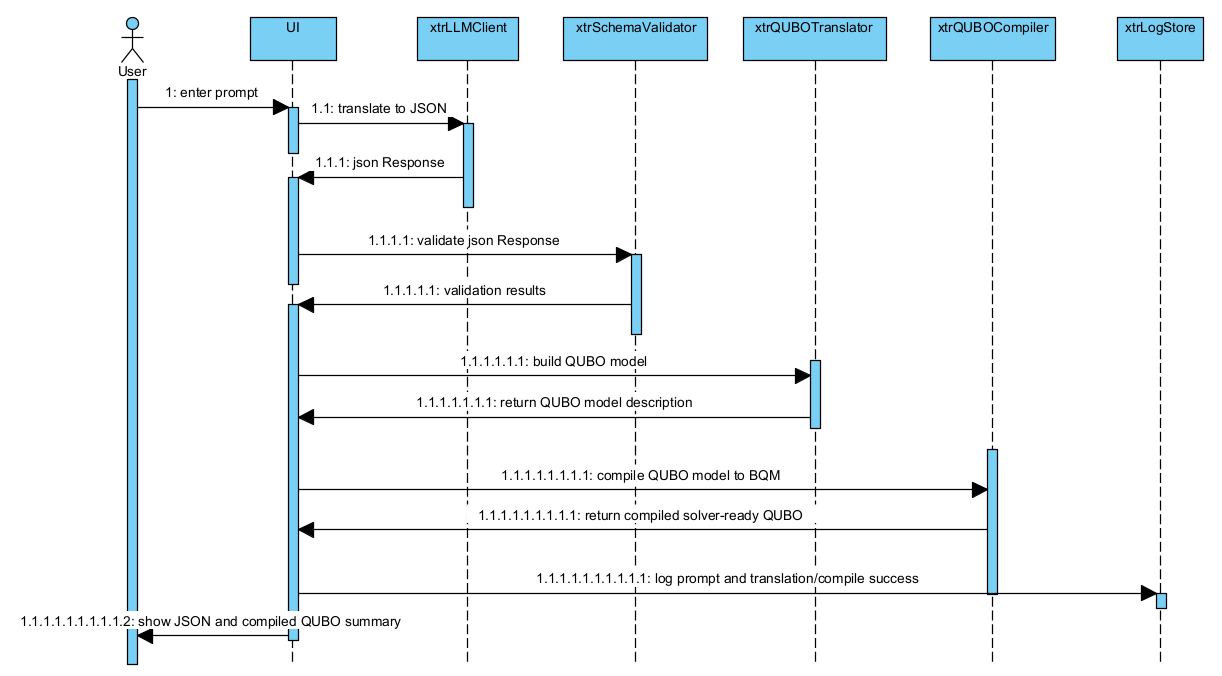
\includegraphics[width=0.95\linewidth]{png/SDUC1.png}
    \caption{Sequence Diagram for \UseCaseNameWIReference{ucTranslatePrompt}}
    \label{fig:uc1-seq}
\end{figure}




\begin{figure}[H]
    \centering
    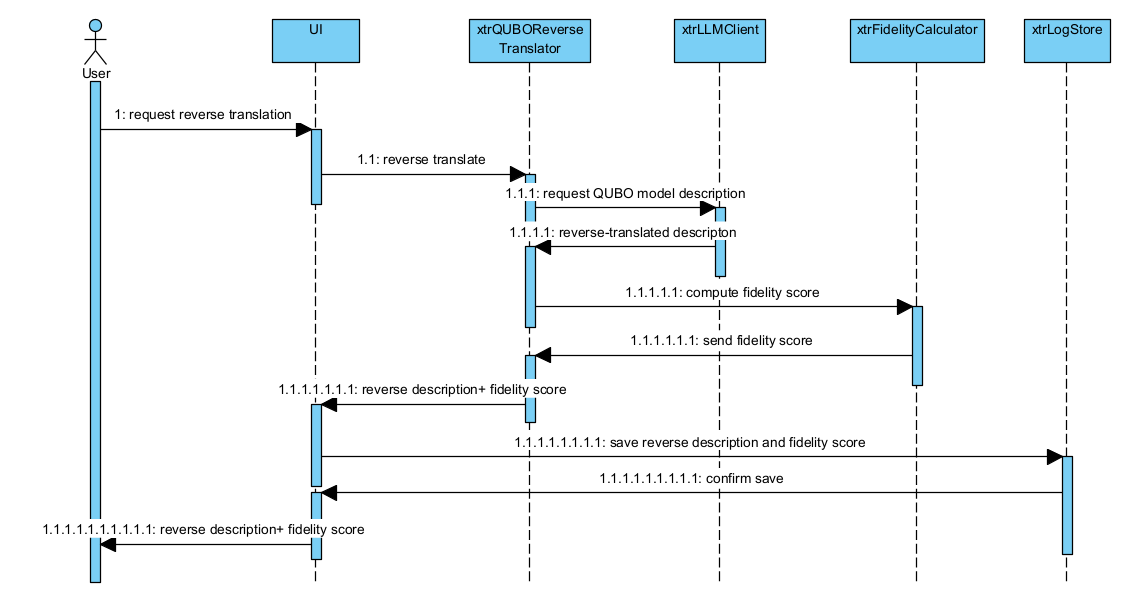
\includegraphics[width=0.95\linewidth]{png/SDUC2.png}
    \caption{Sequence Diagram for  \UseCaseNameWIReference{ucReverseTranslate}}
    \label{fig:uc2-seq}
\end{figure}





\begin{figure}[H]
    \centering
    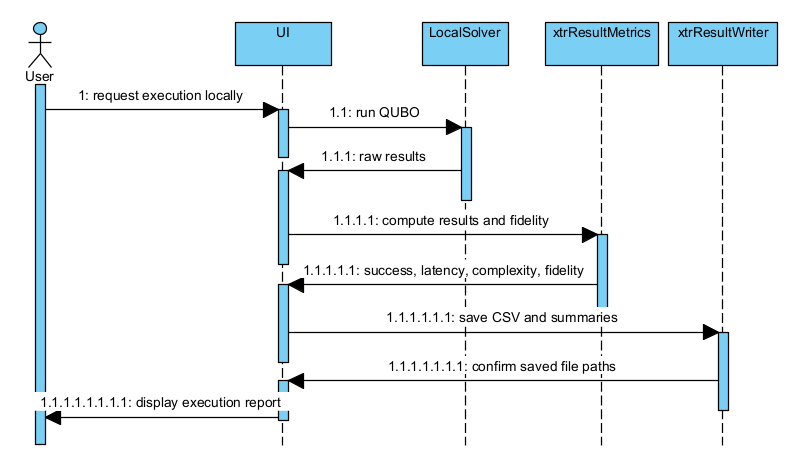
\includegraphics[width=0.95\linewidth]{png/SDUC3.png}
    \caption{Sequence Diagram for \UseCaseNameWIReference{ucExecuteReport}}
    \label{fig:uc3-seq}
\end{figure}

\begin{figure}[H]
    \centering
    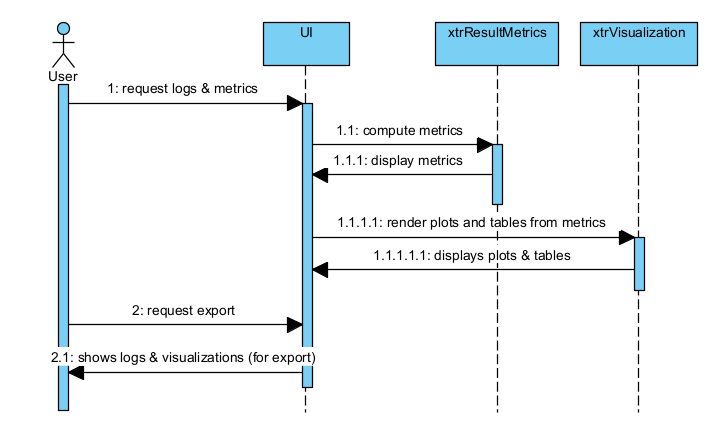
\includegraphics[width=0.95\linewidth]{png/SDUC4.png}
    \caption{Sequence Diagram for \UseCaseNameWIReference{ucViewLogsMetrics}}
    \label{fig:uc4-seq}
\end{figure}

\clearpage
